\section{Tournament Analysis}\label{tournament-analysis}

\subsection{Mean Scores and Coefficient of
Variation}\label{mean-scores-and-coefficient-of-variation}

The tournament is run by considering different number of dancers and
friends. Mean scores and coefficient of variation (standard deviation /
mean) of for various teams is shown in figure \ref{img-mean-cov}.

\begin{figure}[htbp]
\centering
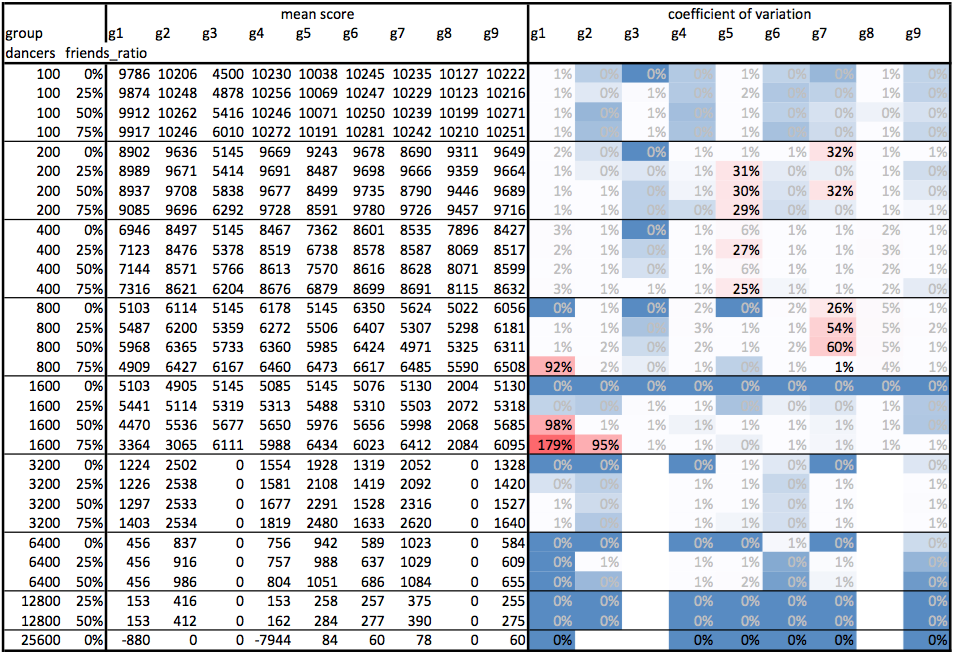
\includegraphics{imgs/mean-cov.png}
\caption{Mean Scores and Coefficient of Variation\label{img-mean-cov}}
\end{figure}

We note that the variation for configurations is generally pretty low (
\(< 1\%\) ). For our group, g2, we notice a huge variation of 95\% for
1600 dancers and 75\% friend density. On further investigating we notice
the following distribution for the given bucket:

\begin{verbatim}
df1[(df1.dancers == 1600)&(df1.friends == 1200)&(df1.group == 'g2')]
\end{verbatim}

\begin{longtable}[c]{@{}lrrcr@{}}
\toprule
& dancers & friends & group & score\tabularnewline
\midrule
\endhead
1791 & 1600 & 1200 & g2 & 6024\tabularnewline
1792 & 1600 & 1200 & g2 & 141\tabularnewline
1793 & 1600 & 1200 & g2 & 5925\tabularnewline
1794 & 1600 & 1200 & g2 & 141\tabularnewline
1795 & 1600 & 1200 & g2 & 141\tabularnewline
1796 & 1600 & 1200 & g2 & 5967\tabularnewline
1797 & 1600 & 1200 & g2 & 141\tabularnewline
1798 & 1600 & 1200 & g2 & 141\tabularnewline
1799 & 1600 & 1200 & g2 & 6017\tabularnewline
1800 & 1600 & 1200 & g2 & 6016\tabularnewline
\bottomrule
\end{longtable}

We try to estimate the friend density for our Medium Strategy and based
on it, we dance with partners for longer duration of time if we think we
have more friends. This gamble does not seem to pay off. We get a
competitive score of 5989.80 in half the scenarios and a meagre 141 for
the rest. We can interpret the result it to state that there is still a
50\% chance that the worst case dancer will not be able to find friends
and dance with them. Because of the uncertainity involved, we would have
been better off just ignoring friends and trying to ensure that every
dancer dances.

We also notice that other players like g1 and g7 also see a huge
variation because of claustrophobia. Other high variations are due to
single outliers (on the worse side) in data.

\begin{verbatim}
df1[df1.score < 0]
\end{verbatim}

\begin{longtable}[c]{@{}lrrcr@{}}
\toprule
& dancers & friends & group & score\tabularnewline
\midrule
\endhead
1360 & 800 & 200 & g7 & -3230\tabularnewline
1437 & 800 & 400 & g7 & -2776\tabularnewline
1468 & 800 & 600 & g1 & -8686\tabularnewline
1702 & 1600 & 800 & g1 & -8688\tabularnewline
1781 & 1600 & 1200 & g1 & -8687\tabularnewline
1782 & 1600 & 1200 & g1 & -8686\tabularnewline
2388 & 25600 & 0 & g1 & -880\tabularnewline
2391 & 25600 & 0 & g4 & -7944\tabularnewline
\bottomrule
\end{longtable}

\subsection{Team wise Scores}\label{team-wise-scores}

After noting that generally the variations are low and that scores
increasing with ratio of friends as a general trend, we decide to take
an average across number of friends to evaluate the performance of each
team. We also categorize the tournament in three categories:

\begin{itemize}
\tightlist
\item
  Small

  \begin{itemize}
  \tightlist
  \item
    for \(d<=800\)
  \item
    It is possible to systematically find soulmates
  \end{itemize}
\item
  Medium

  \begin{itemize}
  \tightlist
  \item
    for \(800 < d <=1600\)
  \item
    It is possible for all dancers to dance at the same time on the
    dance floor
  \end{itemize}
\item
  Large

  \begin{itemize}
  \tightlist
  \item
    for \(1600 < d\)
  \item
    We require some sort of scheduling to ensure each of the dancer gets
    to dance
  \item
    none of the dancers should suffer claustrophobia
  \end{itemize}
\end{itemize}

\begin{figure}[htbp]
\centering
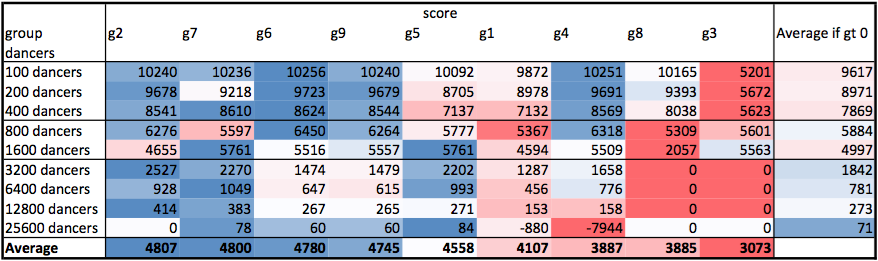
\includegraphics{imgs/team-scores.png}
\caption{Scores of teams per number of dancers\label{team-scores}}
\end{figure}

Figure \ref{team-scores} shows the results for each of the
configuration. We color each row with a heat map, blue being better
score. \textbf{Our group (g2) scores the best Average}, closely followed
by g7. Next best score is by g6 and g9, which share a rather noticable
correlation! We notice the following kinds of teams:

\begin{itemize}
\tightlist
\item
  g1 and g7

  \begin{itemize}
  \tightlist
  \item
    score well on all categories
  \item
    thus score highest and second higher respectively
  \end{itemize}
\item
  g6, g9, g4

  \begin{itemize}
  \tightlist
  \item
    score well on small category
  \end{itemize}
\item
  g5

  \begin{itemize}
  \tightlist
  \item
    scores well on Large category
  \item
    but fails to perform on Small
  \end{itemize}
\end{itemize}

We normalize the scores based on an average of positive scores in each
category in \ref{team-rel} and plot a curve to see the development of
scores with number of dancers for the top 5 teams as shown in figure
\ref{team-5-rel}.

\begin{figure}[htbp]
\centering
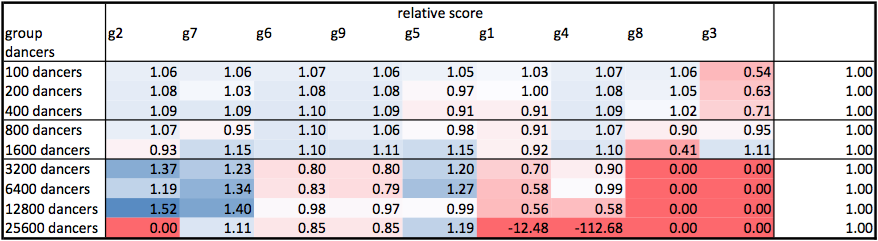
\includegraphics{imgs/team-rel.png}
\caption{Relative scores of teams per number of dancers\label{team-rel}}
\end{figure}

\begin{figure}[htbp]
\centering
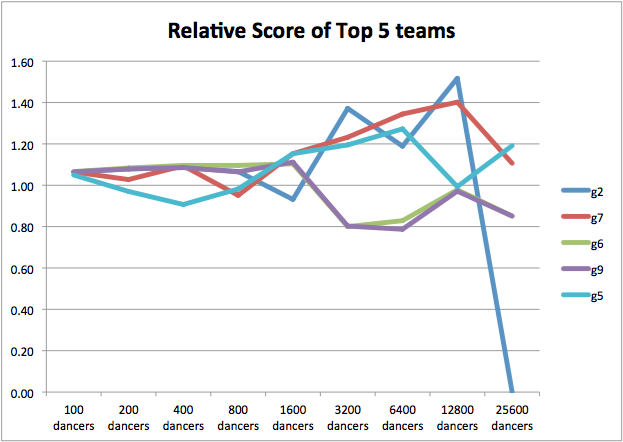
\includegraphics{imgs/team-5-rel.png}
\caption{Plot of relative scores of top 5 teams\label{team-5-rel}}
\end{figure}

As you may notice, the strength of our group is the relatively stronger
scores in Large category. But to decide an ordering, we still follow a
simple average, which seems to favor Small category. Even so, we achieve
the highest overall average, which is testimony to our performance
across categories.

For Large category, our strategy has step behavior. Where as g7 has a
more continuous looking behavior. We present the values of number of
dancers vs maximum dancers without creating claustrophobia.
